

深入研究C++20的细节之前,先简单介绍一下C++20的特性。

这有两个目的:为了给人留下第一印象,并提供相关部分的链接,也可以直接了解细节。本章只有代码片段,而没有完整的程序。

本书一开始就简要介绍了以前的C++标准。比较C++20和以前的版本时,并通过提供历史背景说明了C++20的重要性。

\begin{center}
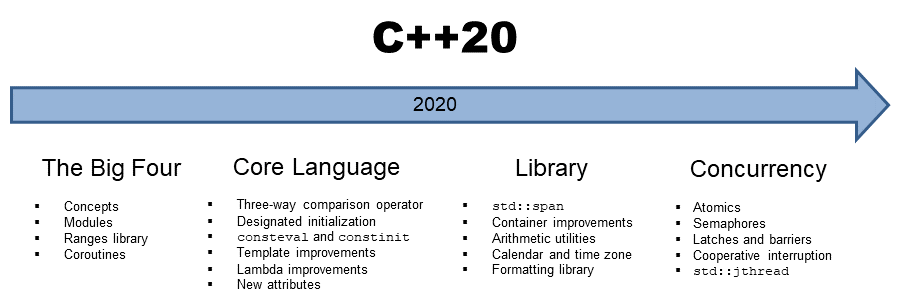
\includegraphics[width=1.0\textwidth]{content/2/chapter3/images/1.png}\\
\end{center}

C++20有四个突出的特性:概念、范围、协程和模块。每个都有自己独立的章节。








